\providecommand{\main}{..}
\documentclass[\main/main.tex]{subfiles}
\begin{document}
\section{Correlation table after removing highly correlated data}
After having removed from the dataset metrics \textbf{CpGobsExp}, \textbf{CpGperCpG}, \textbf{dbVARCount} and \textbf{mamPhyloP46way} looks like:

\begin{figure}
  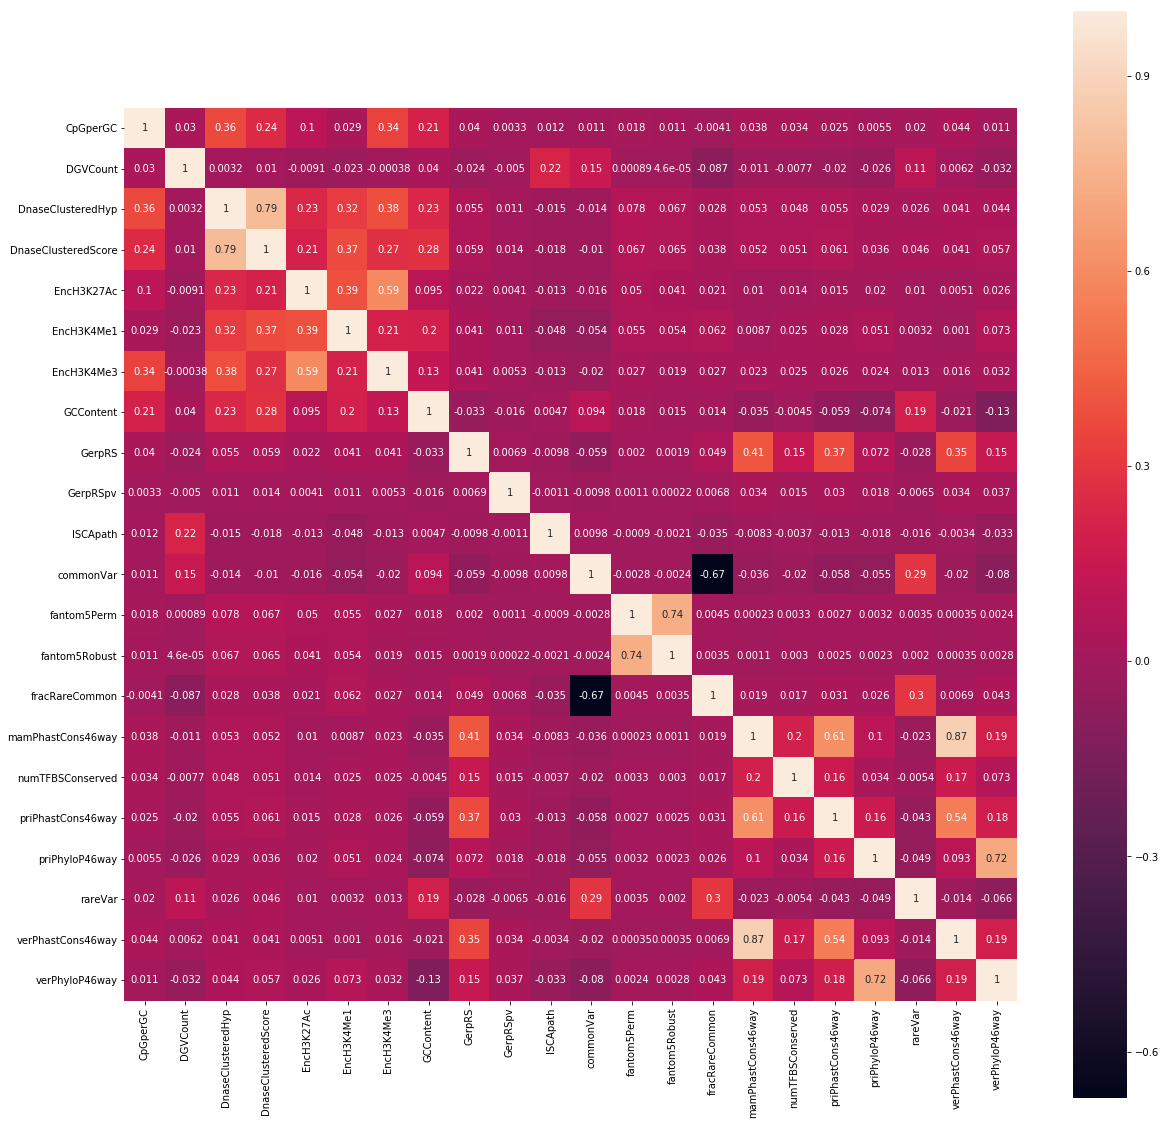
\includegraphics[width=\textwidth]{less_correlated_correlation_matrix}
  \caption{Correlation matrix}
\end{figure}

This correlation matrix with higher resolution is available in the project repository.
\end{document}